% !Mode:: "TeX:UTF-8"

\chapter{}
\textbf{
Consider the Minimum Spanning Tree Problem on an undirected graph $G=(V,E)$, with a cost $c_e\leq 0$ on each edge, where the costs may not all be different. If the costs are not all distinct, there can in general be many distinct minimum-costs solutions. Suppose we are given a spanning tree $T\subseteq E$ with the guarantee that for every $e\in T$, $e$ belongs to \emph{some} minimum-cost spanning tree in $G$. Can we conclude that $T$ itself must be a minimum-cost spanning tree in $G$? Give a proof or a counterexample with explanation.
}

\hspace*{\fill} \\

\noindent
$T$ may not be a minimum-cost spanning tree in $G$.

Let us consider the following instance shown in Fig~\ref{fig_5_1}.
\begin{figure}[!htbp]
\centering
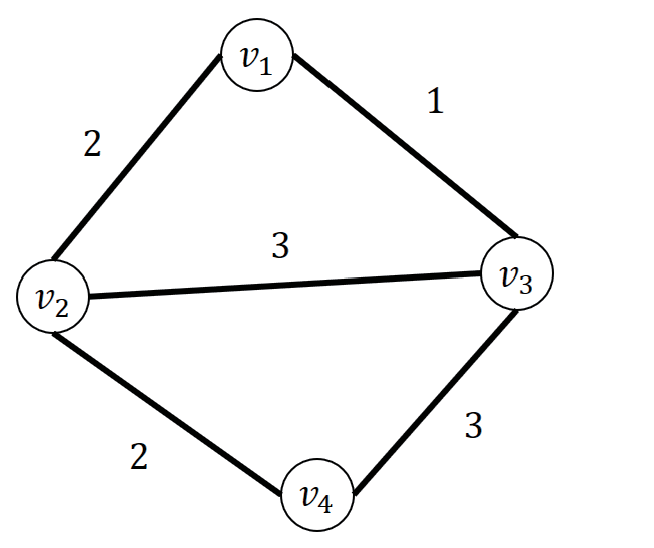
\includegraphics[width=0.5\textwidth]{figures/3.eps}
\caption{An counterexample}\label{fig_5_1}
\end{figure}
Two of its minimum spanning trees are shown in Fig~\ref{fig_5_2}.
\begin{figure}[!htbp]
\centering
\subfigure[minimum spanning tree]{
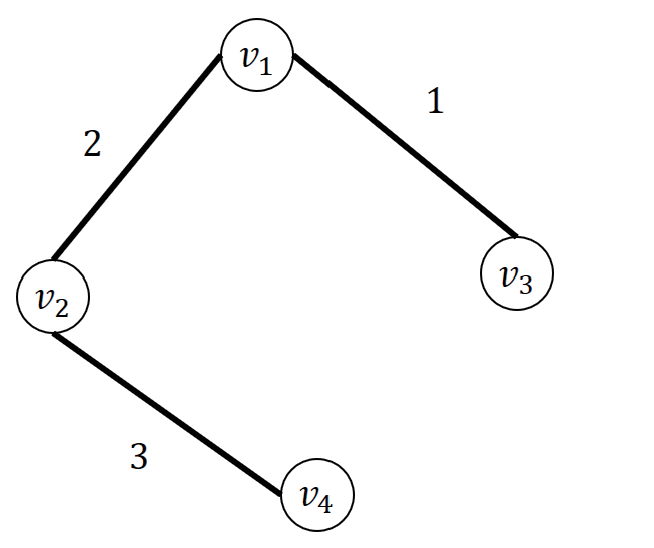
\includegraphics[width=0.46\textwidth]{figures/4.eps}}
\subfigure[minimum spanning tree]{
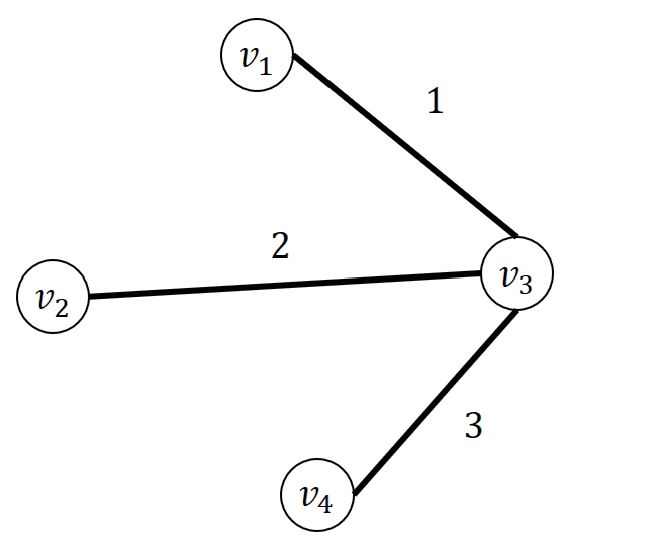
\includegraphics[width=0.46\textwidth]{figures/5.eps}}
\caption{minimum spanning tree. (a)minimum spanning tree 1.
(b)minimum spanning tree 2.}\label{fig_5_2}
\end{figure}
Then we illustrate an example shown in Fig~\ref{fig_5_3}. It is not a minimum-costs spanning tree.
\begin{figure}[!htbp]
\centering
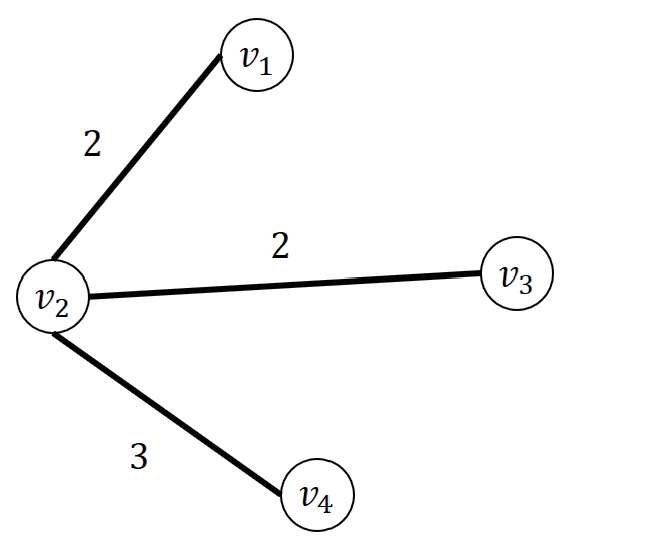
\includegraphics[width=0.5\textwidth]{figures/6.eps}
\caption{An counterexample}\label{fig_5_3}
\end{figure}


